\section{Retas e Planos}

\subsection*{Equação Paramétrica da Reta}


\begin{frame}[label=retas]{Equação Paramétrica de uma Reta}

Fixados um ponto ${\color{red} A}$ de uma reta $r$ e um vetor ${\color{blue}\vec{v}}$ paralelo a esta reta, podemos descrever os pontos $P$ dessa reta da seguinte forma:
\[P={\color{red}A}+t{\color{blue}\vec{v}},\ t\in \R.\]
	\begin{center}
		\begin{tikzpicture}
		\tikzset{>=latex}
		\draw[thick] (-1,-1) -- (2,2);
		\node[left] at (2,2) {r};
		\draw[fill=red] (0,0) circle [radius=1.5pt];
		\node[above left] at (0,0) {$\textcolor{red}{A}$};
		\draw[thick, blue,->] (2,0) -- (0.7+2,0.7);
		\node[blue, right] at (0.7+2,0.7) {$\vec{v}$};
		\onslide<2->{
		\draw[fill=black] (1.5,1.5) circle [radius=1.5pt];
		\node[above left] at (1.5,1.5) {$P$};}
	
	\onslide<3->{
\draw[thick, blue,->] (0,0) -- (1.5,1.5);	
  }
		\end{tikzpicture}
	\end{center}
	
Esta equação é dita {\color{blue} equação vetorial paramétrica da reta $r$}, $t$ é dito ser um {\color{blue}parâmetro} e ${\color{blue}\vec{v}}$ é chamado de {\color{blue}vetor diretor.}

\end{frame}

\begin{frame}[label=retas]
Se	$P=(x,y)$, $\textcolor{red}{A=(x_0,y_0)}$ e $\textcolor{blue}{\vt{v}=(a,b)}$
em coordenadas temos que
\[	\left\{\begin{array}{l}
	x=\textcolor{red}{x_0}+\textcolor{blue}{a}t\\
	y=\textcolor{red}{y_0}+\textcolor{blue}{b}t,\  t\in \R.
	\end{array}\right.\]


Analogamente, se 	$P=(x,y,z)$, $\textcolor{red}{A=(x_0,y_0,z_0)}$ e $\textcolor{blue}{\vt{v}=(a,b,c)}$
		\[	\left\{\begin{array}{l}
		x=\textcolor{red}{x_0}+\textcolor{blue}{a}t\\
		y=\textcolor{red}{y_0}+\textcolor{blue}{b}t\\
		z=\textcolor{red}{z_0}+\textcolor{blue}{c}t,\  t\in \R.
		\end{array}\right.\]
		Estas equações são chamadas simplesmente de \dest{equações paramétricas  da reta} $r$.


\end{frame}

\begin{frame}[label=retas]
	\frametitle{ }
	%\begin{scriptsize}
	{\begin{exe}\label{exer4} \noindent
			
			\begin{enumerate}[a]
				\item Determine as equações paramétricas da reta que passa pelos pontos  $A=(-1,0)$ e $B=(0,1)$ .
				
				\item Determinar  as equações paramétricas da reta $r$ que passa pelos
				pontos $A = (1, 2, -2)$ e $B = (-1, 4, 2)$.

	\item\label{ex6} Sejam $A=(0,1,8), B=(-3,0,9)$ e $r: X=(1,2,0)+t(1,1,-3)$. Determine o ponto $C$ de $r$ tal que $A,B$ e $C$ sejam vértices de um triângulo retângulo com ângulo reto no vértice $A$.
			\end{enumerate}
	\end{exe}}

\end{frame}

\begin{frame}[label=retas]
	\begin{casa}
	\begin{enumerate}
		\item 	Considere os pontos $A = (2, -1, 0)$,  $B  = (0, 1, -1)$. Determine
	 a reta $r$ que passa por $A$ e $B$.

	\item Sejam $A=(0,1,8), B=(-3,0,9)$ e $r: X=(1,2,0)+t(1,1,-3)$. Determine o ponto $C$ de $r$ tal que $A,B$ e $C$ sejam vértices de um triângulo retângulo com ângulo reto no vértice $C$. 
	\end{enumerate}
	
	\end{casa}

	
\begin{center}
\begin{block}{}
Note que a equação vetorial paramétrica da reta é válida para qualquer dimensão!
\end{block}
\end{center}
\end{frame}

\subsection*{Equações Cartesianas da reta em $\R^2$}
\begin{frame}[label=retas]{Equação Cartesiana da reta em $\R^2$}
	Fixe um ponto $\textcolor{red}{A=(x_0,y_0)}$ de uma reta $r$ e seja  $\textcolor{blue}{\vt{v}=(a,b)}$ um vetor ortogonal a esta reta. 
	
		\begin{center}
		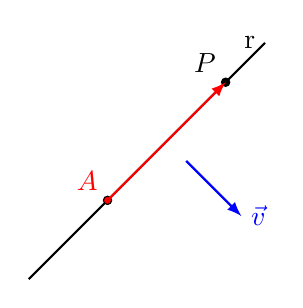
\begin{tikzpicture}
		\tikzset{>=latex}
		\draw[thick] (-1,-1) -- (2,2);
		\node[left] at (2,2) {r};
		
		\draw[thick, blue,->] (1,0.5) -- (0.7+1,-0.7+0.5);
		\node[blue, right] at (0.7+1,-0.7+0.5) {$\vec{v}$};
		\draw[fill=red] (0,0) circle [radius=1.5pt];
		\node[above left] at (0,0) {$\textcolor{red}{A}$};
		\onslide<1->{
			
			\draw[fill=black] (1.5,1.5) circle [radius=1.5pt];
			\node[above left] at (1.5,1.5) {$P$};}
		
		\onslide<1->{
			\draw[thick, red,->] (0,0) -- (1.5,1.5);	
		}
		\end{tikzpicture}
	\end{center}
	
Dado um ponto qualquer   $P=(x,y)$	desta reta $r$  temos que
		\[	\textcolor{blue}{a}x+\textcolor{blue}{b}y+c=0.\]
Esta equação é dita \dest{equação cartesiana da reta}.
\end{frame}
	
\begin{frame}[label=retas]
	\begin{exe}\noindent
  Encontre a equação cartesiana da reta que passa pelos pontos $P=(1,3)$ e $Q=(5,-9)$.
	\end{exe}

	\begin{block}{Equação reduzida da reta}
		A equação cartesiana de uma reta é chamada de   \dest{equação reduzida} quando  está na seguinte forma:
		\[y=mx+n.\]
		O coeficiente  $m$ é dito \dest{coeficiente angular} da reta e mede a tangente do ângulo que a reta faz com o eixo $OX$. E o número $n$ é dito \dest{coeficiente linear} da reta e representa a ordenada do ponto de interseção da reta com o eixo $OY$.
	\end{block}

\end{frame}

\begin{frame}
	
	%\begin{scriptsize}
	\begin{block}{Equação segmentária da reta}
		A equação cartesiana de uma reta é chamada de   \dest{equação segmentária}  quando  está na seguinte forma:
		\[\frac{x}{p}+\frac{y}{q}=1.\]
		Neste caso, a reta intercepta os eixos $OX$ e $OY$ nas coordenadas $p$ e $q$ respectivamente. 
	\end{block}
	
	%\end{scriptsize}
\end{frame}

\begin{frame}
	\begin{exe}
	\begin{enumerate}
		\item 	 Determine a equação cartesiana da reta $r$ que passa pelos pontos $A=(0,3)$ e $B=(2,0)$.
		
		
		\item Determine a equação cartesiana da reta que passa pelos pontos $A=(0,1)$ e $B=(2,2)$.
		
		
	\end{enumerate}
	\end{exe}


	\begin{minipage}{0.45\textwidth}
		\begin{figure}[h]
		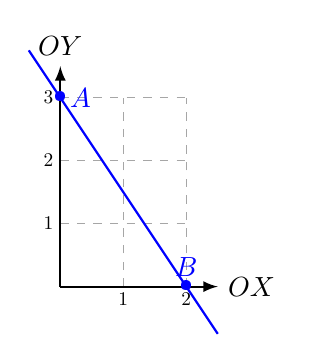
\begin{tikzpicture}[scale=0.8]
	\tikzset{>=latex}
	\draw[help lines, color=gray!70, dashed] (0,0) grid (2,3);
	\draw[->,thick] (0,0)--(2.5,0) node[right]{$OX$};
	\draw[->,thick] (0,0)--(0,3.5) node[above]{$OY$};
	\foreach \i in {1,...,2}
	\node[below,scale=0.7] at (\i,0) {$\i$};
	\foreach \i in {1,...,3}
	\node[left,scale=0.7] at (0,\i) {$\i$};
	
	
	\coordinate (O) at (0,0);
	\coordinate (A) at (0,3);
	\coordinate (B) at (2,0);
	
	
	\node[blue] at (A) {\textbullet};
	\node[blue,right] at (A) {$A$};
	
	\node[blue] at (B) {\textbullet};
	\node[blue,above] at (B) {$B$};
	
	\draw[blue,thick] (-.5,3.75) -- (2.5,-0.75) ;
	
	
	
	%	\node[blue] at (Q) {\textbullet};
	%	\node[blue,above] at (Q) {$Q$};
	
	\end{tikzpicture}
	\caption{Exemplo 1}
	\end{figure}
	\end{minipage}
	\begin{minipage}{0.45\textwidth}
		\begin{figure}[h]
	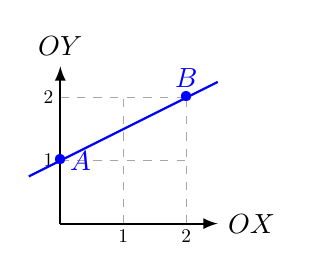
\begin{tikzpicture}[scale=0.8]
	\tikzset{>=latex}
	\draw[help lines, color=gray!70, dashed] (0,0) grid (2,2);
	\draw[->,thick] (0,0)--(2.5,0) node[right]{$OX$};
	\draw[->,thick] (0,0)--(0,2.5) node[above]{$OY$};
	\foreach \i in {1,...,2}
	\node[below,scale=0.7] at (\i,0) {$\i$};
	\foreach \i in {1,...,2}
	\node[left,scale=0.7] at (0,\i) {$\i$};
	
	
	\coordinate (O) at (0,0);
	\coordinate (A) at (0,1);
	\coordinate (B) at (2,2);
	
	
	\node[blue] at (A) {\textbullet};
	\node[blue,right] at (A) {$A$};
	
	\node[blue] at (B) {\textbullet};
	\node[blue,above] at (B) {$B$};
	
	\draw[blue,thick] (-.5,0.75) -- (2.5,2.25) ;
	
	
	
	%	\node[blue] at (Q) {\textbullet};
	%	\node[blue,above] at (Q) {$Q$};
	
	\end{tikzpicture}
	\caption{Exemplo 2}
\end{figure}
	\end{minipage}


\end{frame}

\begin{frame}[label=retas]
\begin{casa}
	\begin{enumerate}
		\item Determine a equação da reta que passa pelo ponto $A=(3,-5)$ e tem coeficiente angular igual a $5$.
		
		\item Esboce no plano a reta cuja equação é dada por $\frac{x}{-3}+\frac{y}{2}=1$.
	\end{enumerate}
\end{casa}
\end{frame}

\subsection*{Equação Cartesiana do Plano no Espaço}

\begin{frame}[label=planos]{Equação Cartesiana do Plano no Espaço}
Sejam  ${\color{red}A=(x_0,y_0,z_0)}$  um ponto de um plano em $\R^3$, $\textcolor{blue}{\vt{n}=(a,b,c)}\perp \pi$, então os pontos e  $P=(x,y,z)$do plano devem satisfazer a seguinte \dt{equação cartesiana}
\[{\color{blue}a}x+{\color{blue}b}y+{\color{blue}c}z+{\color{red}d}=0\]
\begin{center}
\includegraphics[scale=0.8]{figuras/normal-vector.png}
\end{center}
\end{frame}

\begin{frame}
\begin{exe}
Determine a equação do plano que passa pelo ponto $A=(1,0,1)$ e é perpendicular à reta
$r: X=(-1,1,2)+t(0,2,1),\ t\in \R$.
\end{exe}

\end{frame}

\begin{frame}[label=sistemas,fragile=singleslide]{Interseção de Planos}

\begin{pycode}
import sympy as sp

x,y,z=sp.symbols('x y z',real=True)
X=sp.Matrix([x,y,z])
A=sp.Matrix([[2, -1,1],[1,3,4]])
B=sp.Matrix([2,1])
AX=A*X
eq1=sp.Eq(AX[0],B[0])
eq2=sp.Eq(AX[1],B[1])

sol=sp.solve(sp.Eq(AX,B),(x,y,z))

\end{pycode}


Qual o conjunto dos pontos do espaço que estão na interseção dos dois planos a seguir?

\[\begin{cases}
\pyl{eq1}\\
\pyl{eq2}
\end{cases}\]
Para descobrir isso, vemos multiplicar a 2\fm equação por $-2$ e somar com a primeira.
\[\begin{cases}
\pyl{eq1}\\
\pyl{-2*AX[1]+AX[0]}=\pyl{-2*B[1]+B[0]}
\end{cases}\]
Note que geometricamente os dois sistemas tratam de interseção de planos diferentes, mas algebricamente os sistemas são {\color{blue} equivalentes}, isto é, têm o mesmo conjunto de pontos $(x,y,z)$ como solução. Entretanto o segundo sistema é mais simples!
\end{frame}


\begin{frame}[label=sistemas,fragile=singleslide]

\begin{pycode}
import sympy as sp

x,y,z=sp.symbols('x y z',real=True)
X=sp.Matrix([x,y,z])
A=sp.Matrix([[2, -1,1],[1,3,4]])
B=sp.Matrix([2,1])
AX=A*X
eq1=sp.Eq(AX[0],B[0])
eq2=sp.Eq(AX[1],B[1])

sol=sp.solve(sp.Eq(AX,B),(x,y,z))

\end{pycode}

\[\begin{cases}
\pyl{eq1}\\
\pyl{-2*AX[1]+AX[0]}=\pyl{-2*B[1]+B[0]}
\end{cases}\]
É fácil ver que este sistema tem soluções da forma:
\[y=\pyl{sol[y]} \text{ e } x=\pyl{sol[x]}.\]
Fazendo $z=t$, vemos que os pontos da interseção são da forma
\[X=(1-t,-t,t)=(1,0,0)+t(-1,-1,1)\ t \in \R,\]
isto é, uma reta em $\R^3$. 
\medskip

Isto nos motiva a estudar os chamados {\color{blue}sistemas lineares}.

\end{frame}










